\chapter{Projekt}
\subsection{Architektura projektu}
Cieżko jest mówić o naszej aplikacji jak o jednym bycie, ponieważ można ją podzielić na dwa podsystemu, gdzie w obu przypadkach archiktektura systemu jest wielowarstwowa. Jednym z podsystemów jest aplikacja webowa, która została zaprojektowana w oparciu o wzorzec \textbf{MVC} (ang. Model-View-Controller), który to narzucił wielowarstwową architektura. Oddzielając logikę biznesową od modelu (tj. danych) oraz interfejsu użytkownika aplikacji została zaprojektowana zgodnie z zasadami \textbf{GRASP} (ang. General responsibility assignment software patterns). Taka a nie inna architektura aplikacji webowej oprócz znacznego zwiększenia czytelności kodu pozwoliła na wielowarstwowe zabezpieczenia, które zostały nałożone na każdą z trzech głównych warstw naszej aplikacji. Samą część łącząca wartswe modelu oraz controller'a możemy podzielić na dwie podwarstwy: \textbf{DAO} (ang. Data Access Object) oraz \textbf{Service}.
\begin{figure}[H]
  \centering
  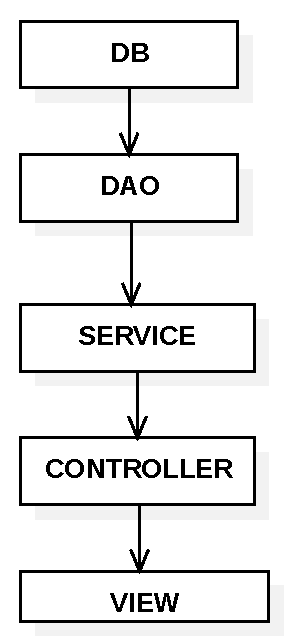
\includegraphics[scale=0.6]{diagram1.pdf}
  \caption{System podzielony na podwarstwy.}
\end{figure}
Warstwa \textbf{DAO} odpowiedzialna jest bezpośrednio na komunikacje z wartswą modelu, tj. bazą danych. Natomiast to w warstwie serwisowej, która korzysta z warstwy \textbf{DAO} została zaimplementowana cała logika biznesowa i to właśnie z warstwy serwisowej korzystamy w kontrolerach.

\paragraph{}
Drugim podsystemem naszego projektu jest aplikacja webowa, która również jest systemem rozproszonym komunikującym się z serwerem (który jest częścią pierwszego podsystemu) wykorzystując \textbf{REST} (ang. Representational State Transfer) oferując użytkownikowi jedynie część funkcjonalności aplikacji webowej.

\paragraph{}
W projekcie poza stosowaniem zasad \textbf{GRASP} zostały wykorzystane takie wzorce projektowe jak \textbf{Proxy}, \textbf{Template Method}, \textbf{Adapter}, \textbf{Factory} oraz \textbf{Decorator}, \textbf{Dependency Injection}, \textbf{Aspect Oriented Programing}, \textbf{Singleton}, które w sposób naturalny współgrały z użytymi przez nas technologiami.
\subsection{Przypadki użycia i scenariusze}
\begin{table}[H]
	\centering
	\sffamily\captionsetup{justification=raggedright,singlelinecheck=false,position = below, font = sf}
	\begin{tabular}{|m{3.5cm}|m{11cm}|}
	\hline 
	UC1 & Add Survey \\
	\hline
	Actors & Company \\ 
	\hline
	Preconditions & Company is signed in and is in the dashboard page. \\
	\hline
	Postconditions & Company added survey. \\
	\multirow{6}{*}{Main Success Scenario} & 1.Company hits on 'Add Survey' button. \\
	\cline{2-2}
	& 2.Company hits proper 'Add Question' button depending on what type of question company wants. \\
	\cline{2-2}
	& 3.Company fills up question's content. \\
	\cline{2-2}
	& 4.Company repeats steps from point 2. until completes survey. \\
	\cline{2-2}
	& 5.Company hits 'Add Voucher' button in order to compose survey with concere voucher. \\
	\cline{2-2}
	& 6.Company hits 'Confirm Survey' button. \\
	\hline
	\multirow{4}{*}{Alternate flows} & 2a.Company hits 'Confirm Survey' button without adding any questions: \\
	\cline{2-2}
	& \multicolumn{1}{c|}{1.System signals error and doesn't proceed.} \\
	\cline{2-2}
	& 5a.Company hits 'Confirm Survey' button without adding voucher: \\
	\cline{2-2}
	& \multicolumn{1}{c|}{1.System signals error and doesn't proceed.} \\
	\hline	
	\end{tabular}
\end{table}		

\paragraph{}
Powyższy przypadek użycia opisuje proces dodawania ankiety so systemu. Szczegóły dodawania ankiety zostały opisane w rozdziale czwartym.
		
\begin{table}[H]
	\centering
	\sffamily\captionsetup{justification=raggedright,singlelinecheck=false,position = below, font = sf}
	\begin{tabular}{|m{3.5cm}|m{11cm}|}
	\hline
	UC2 & Sign in \\
	\hline
	Actors & Company \\
	\hline
	Preconditions & Company is registered in the System  \\
	\hline
	Postconditions & Company is signed in. \\
	\hline
	\multirow{7}{*}{Main Success Scenario} & 1.Company enters the website and is on landing page \\
    \cline{2-2}
     & 2.Company hits the Sign In button. \\
	\cline{2-2}
     & 3.System moves the Company to the Sign In page.\\
	\cline{2-2}
     & 4.Company enters the login. \\
	\cline{2-2}
     & 5.Company enters the password. \\
	\cline{2-2}
     & 6.Company hits the Sign In/Enter button. \\
	\cline{2-2}
     & 7.System moven the Company to the dashboard page. \\
    \hline
    \multirow{10}{*}{Alternate flows} & 2a.Company hits the Sign Up button: \\
	\cline{2-2}
	& \multicolumn{1}{c|}{1.System moves the Company to the Sign Up page.} \\
	\cline{2-2}
	& 6a.Company hits the Sign Up button or "Doesn't hvae an account? Create one here now!" text. \\
	\cline{2-2}
	& \multicolumn{1}{c|}{1.System moves the Company to the Sign Up page.}	 \\
	\cline{2-2}
	& 6b.Company hits "Forgot the password" text. \\
	\cline{2-2}
	& \multicolumn{1}{c|}{1.Company is guided through password recovery process.} \\
	\cline{2-2}
	& 7a.Invalid login: \\
	\cline{2-2}
	& \multicolumn{1}{c|}{1.System signals error and doesn't proceed/stays on the Sign In page.}	 \\
	\cline{2-2}
	& 7b.Invalid password: \\
	\cline{2-2}
	& \multicolumn{1}{c|}{1.System signals error and doesn't proceed/stays on the Sign In page.} \\
    \hline
	\end{tabular}
\end{table}

\paragraph{}
Powyższy przypadek użycia opisuje proces logowania do systemu. Szczegółowy proces został opisany w rozdziale czwartym.
	
	\begin{table}[H]
	\centering
	\sffamily\captionsetup{justification=raggedright,singlelinecheck=false,position = below, font = sf}
	\begin{tabular}{|m{3.5cm}|m{11cm}|}
	\hline 
	UC3 & Sign up \\
	\hline
	Actors & Company \\
	\hline
	Preconditions & Company is not already registered in the System. \\
	\hline
	Postconditions & Company is registered in the System. Company is able to access its dashboard. \\	
	\hline
	\multirow{8}{*}{Main Success Scenario} & 1.Company enters the website and is on landing page. \\
	\cline{2-2}
	& 2.Company hits the Sign Up button. \\
	\cline{2-2}
	& 3.System moves the Company to the Sign Up page. \\
	\cline{2-2}
	& 4.Company enters login, password, name and address. \\
	\cline{2-2}
	& 5.Company hits Sign Up/Enter button. \\
	\cline{2-2}
	& 6.System notifies Company about successful registration. \\
	\cline{2-2}
	& 7.System moves Company to the landing page. \\
	\cline{2-2}
	& 8. System can also demand entering a verification token from e-mail after the registration. \\
	\hline
	\multirow{10}{*}{Alternate flows} & 2a.Company hits the Sign In button: \\
	\cline{2-2}
	& \multicolumn{1}{c|}{1.System moves the Company to the Sign In page.} \\
	\cline{2-2}
	& 5a.Company hits Cancel/Back button: \\
	\cline{2-2}
	& \multicolumn{1}{c|}{1.System moves the Company to the landing page.} \\
	\cline{2-2}
	& 6a.Login/e-mail already taken: \\
	\cline{2-2}
	& \multicolumn{1}{c|}{1.System signals error and doesn't proceed.} \\
	\cline{2-2}
	& 6b.Login/Name/Address contains forbidden symbols: \\
	\cline{2-2}
	& \multicolumn{1}{c|}{1.System signals error, suggests the proper symbol range and doesn't proceed.} \\
	\cline{2-2}
	& 6c.Any of registration fields is empty: \\
	\cline{2-2}
	& \multicolumn{1}{c|}{1.System signals error, suggests to fill the empty field and doesn't proceed.} \\
	\hline
	\end{tabular}
	\end{table}
	
\paragraph{}
Powyższy przypadek użycia opisuje proces rejestracji w systemie. Szczegółowy proces został opisany w rozdziale czwartym.
	
	\begin{table}[H]
	\centering
	\sffamily\captionsetup{justification=raggedright,singlelinecheck=false,position = below, font = sf}
	\begin{tabular}{|m{3.5cm}|m{11cm}|}
	\hline 
	UC4 & Filling up the survey \\
	\hline
	Actors & User \\ 
	\hline
	Preconditions & None or the mobile app installed required , if user want's to make it that way \\
	\hline
	Postconditions & User accomplished fulfilling the survey. User gain a voucher code. \\
	\multirow{10}{*}{Main Success Scenario} & 1.User chose a company, which voucher might be interesting for him (either in mobile app or website). \\
	\cline{2-2}
	& 2.System moves user to website where the survey is shown. \\
	\cline{2-2}
	& 3.User fulfilss whole survey step by step. \\
	\cline{2-2}
	& 4.User hits 'Done' button. \\
	\cline{2-2}
	& 5.System validates survey and user moves forward. \\
	\cline{2-2}
	& 6.System notifies user that the survey is accepted. \\
	\cline{2-2}
	& 7.System asks user for e-mail Adress	 \\
	\cline{2-2}
	& 8.User can aceppt his e-mail Adress by pressing the button.  \\
	\cline{2-2}
	& 9.System sends voucher to user. \\
	\cline{2-2}
	& 10.System notifies user that the voucher has been sent. \\
	\hline
	\multirow{3}{*}{Alternate flows} & 5a.Survey rejected, validation didn't pass: \\
	\cline{2-2}
	& \multicolumn{1}{c|}{1.Special informations are displayed.} \\
	\cline{2-2}
	& \multicolumn{1}{c|}{2.User is asked to fix his answers.} \\
	\cline{2-2}
	\multirow{3}{*}{Alternate flows} & 9a.User passed e-mail that don't match e-mail address' pattern: \\
	\cline{2-2}
	& \multicolumn{1}{c|}{1.Special informations are displayed.} \\
	\cline{2-2}
	& \multicolumn{1}{c|}{2.User is asked to pass proper e-mail address.} \\
	\hline	
	\end{tabular}
	\end{table}	

\paragraph{}
Powyższy przypadek użycia opisuje proces wypełniania ankiety. Szczegółowy proces został opisany w rozdziale czwartym.
	
	
	\begin{table}[H]
	\centering
	\sffamily\captionsetup{justification=raggedright,singlelinecheck=false,position = below, font = sf}
	\begin{tabular}{|m{3.5cm}|m{11cm}|}
	\hline 
	UC5 & Add Voucher \\
	\hline
	Actors & Company \\
	\hline
	Preconditions & Company is signed in and is in dashboard page. \\
	\hline
	Postconditions & Company added voucher. \\	
	\hline
	\multirow{5}{*}{Main Success Scenario} & 1.Company hits „Add voucher” button. \\
	\cline{2-2}
	& 2.Company fills up voucher details( some details in plain text,type of discount, discount rate etc.) \\
	\cline{2-2}
	& 3.Company hits „Add voucher” button to add voucher to right survey from dropdown list. \\
	\cline{2-2}
	& 4.Company confirms voucher by „Confirm voucher” button. \\
	\cline{2-2}
	& 5.Voucher is added. \\
	\hline
	\multirow{6}{*}{Alternate flows} & 5a. Voucher already exist: \\
	\cline{2-2}
	& \multicolumn{1}{c|}{1.Proper error message is displayed.} \\
	\cline{2-2}
	& \multicolumn{1}{c|}{2.Filled for is displayed, company is asked to pass diffrent voucher.} \\
	\cline{2-2}
	& 5b.Company didn't pick any survey: \\
	\cline{2-2}
	& \multicolumn{1}{c|}{1.Proper error message is displayed.} \\
	\cline{2-2}
	& \multicolumn{1}{c|}{2.Filled for is displayed, company is asked to pass diffrent voucher.} \\
	\cline{2-2}
	\hline
	\end{tabular}
	\end{table}
	
\paragraph{}
Powyższy przypadek użycia opisuje proces dodawania kuponu. Szczegółowy proces został opisany w rozdziale czwartym.
	
	\begin{table}[H]
	\centering
	\sffamily\captionsetup{justification=raggedright,singlelinecheck=false,position = below, font = sf}
	\begin{tabular}{|m{3.5cm}|m{11cm}|}
	\hline 
	UC6 & Remove account \\
	\hline
	Actors & Company \\
	\hline
	Preconditions & Company is registered in system. \\
	\hline
	Postconditions & Company doesn’t have an account. \\	
	\hline
	\multirow{5}{*}{Main Success Scenario} & 1.Company hits „Delete account” button \\
	\cline{2-2}
	& 2.Confirmation window appears asking for confirmation. \\
	\cline{2-2}
	& 3.Company confirms the action by entering the password to the site. \\
	\cline{2-2}
	& 4.All information about the company, surveys and coupons are deleted from database. \\
	\cline{2-2}
	& 5.Company sees statement „Your account has been deleted.”. \\
	\hline
	\end{tabular}
\end{table}

\paragraph{}
Powyższy przypadek użyca opisuje proces usuwania konta z systemu. Wraz z usunięciem konta z systemu, z bazy danych są usuwane kaskadowo wszystkie krotki, które były powiązane z danym kontem firmowym.


\subsection{Diagramy klas}
Diagramy przedstawione poniżej przedstawiają klasy serwisowe, w których to właśnie została zaimplementowana cała logika biznesowa naszego systemu  i to one reprezentują funkcjonalność i możliwości naszej aplikacji webowej. W celu zwiększenia czytelności diagramów z ich większości zostały usunięte trywialne metody (nie zawierające logiki biznesowej), których zadaniem było dodanie, edycja, usunięcie przekazywanego obiektu w bazie danych.
\begin{figure}[H]
  \centering
  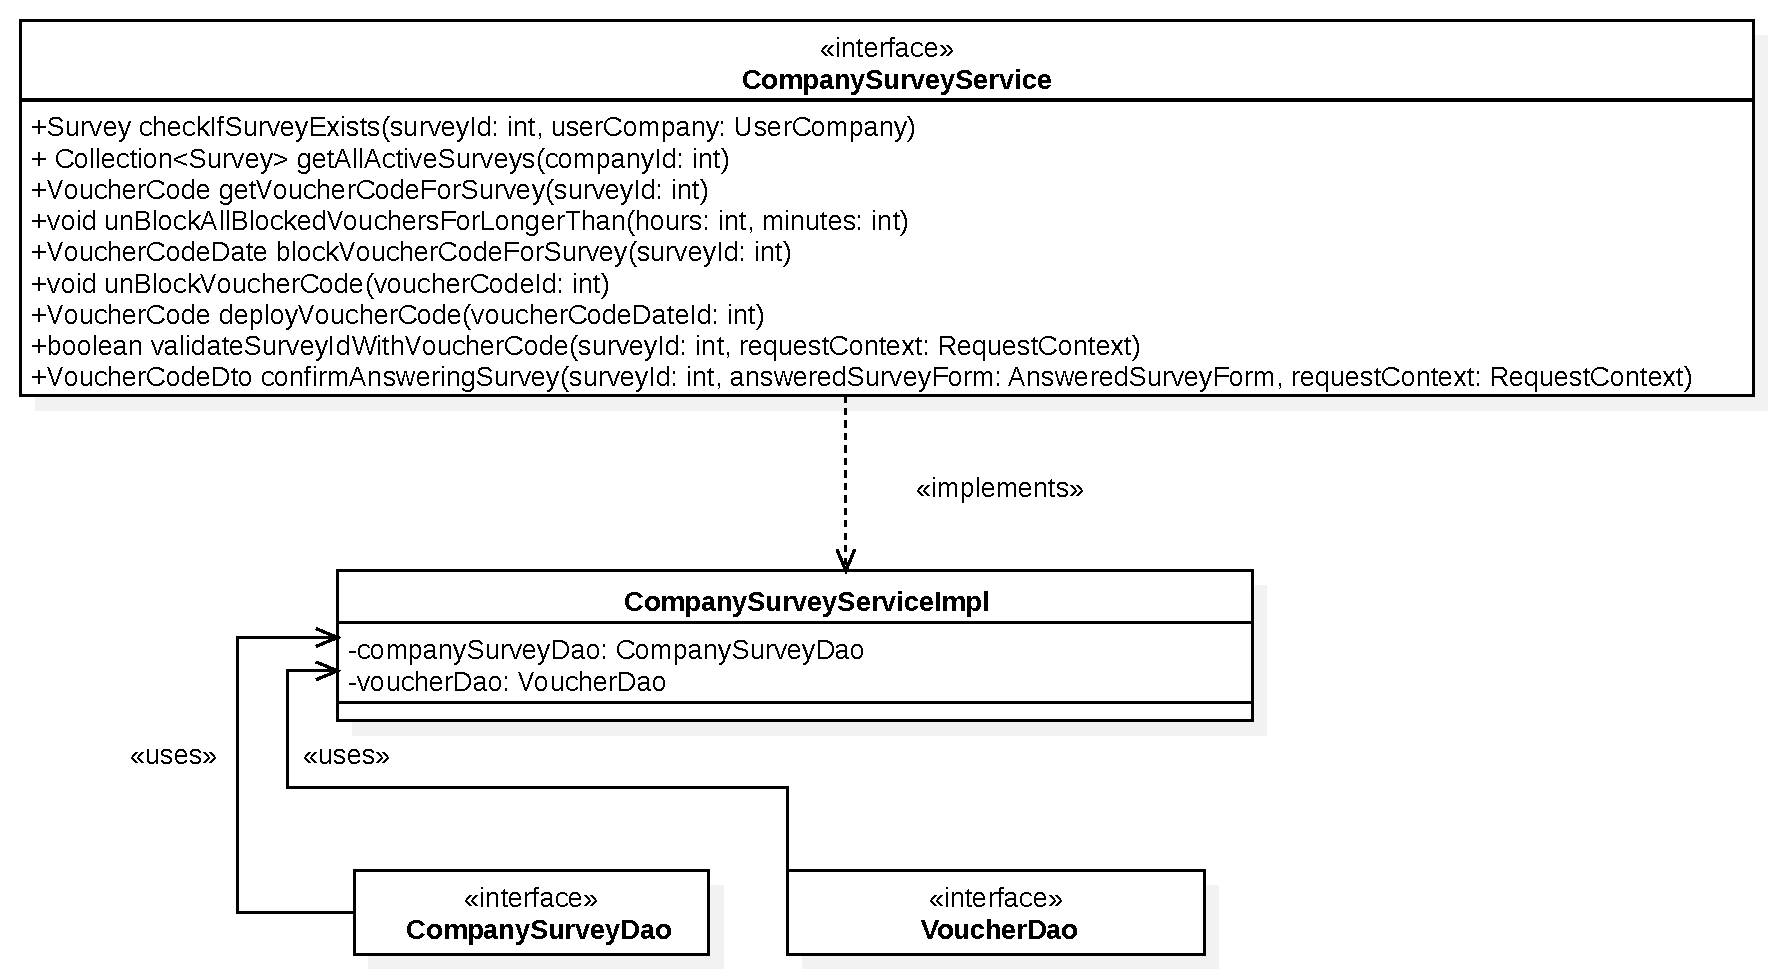
\includegraphics[width=15cm,height=20cm,keepaspectratio]{company_survey_service.pdf}
  \caption{Diagram klas dla interfejsu serwisowego $CompanySurveyService$}
\end{figure}
Powyższy diagram przedstawia diagram klas dla serwisu, który przede wszystskim obsługuje funkcjonalność związana pobieraniem aktywnym, przeglądaniem oraz wypełnianiem ankiet jak również walidacją tych czynności. Ponadto odpowiedzialny jest za podjęcie decyzji czy dany kupon powininen zostać wydany czy też nie.
\begin{figure}[H]
  \centering
  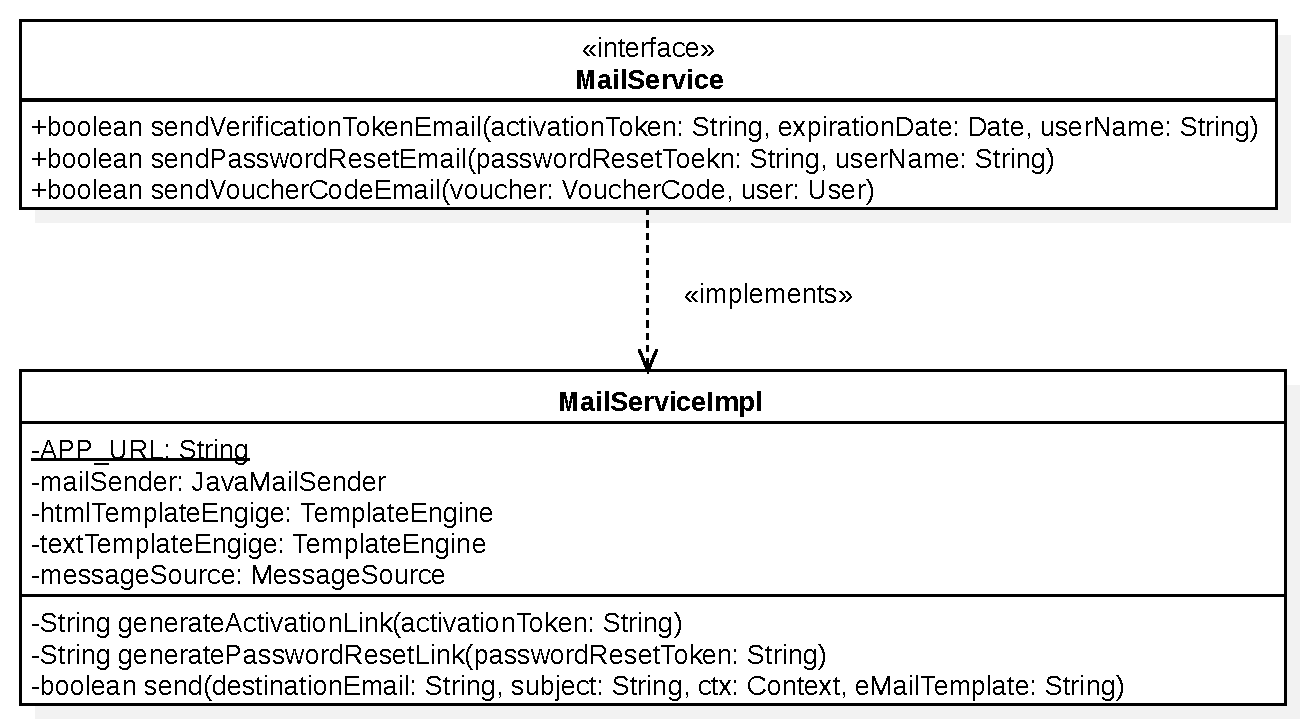
\includegraphics[scale=0.6]{mail_service.pdf}
  \caption{Diagram klas dla interfejsu serwisowego $MailService$}
\end{figure}
W \textbf{MailService} każda metoda odpowiada innemu typu  wiadomości, która zostanie wysłąna.
\begin{figure}[H]
  \centering
  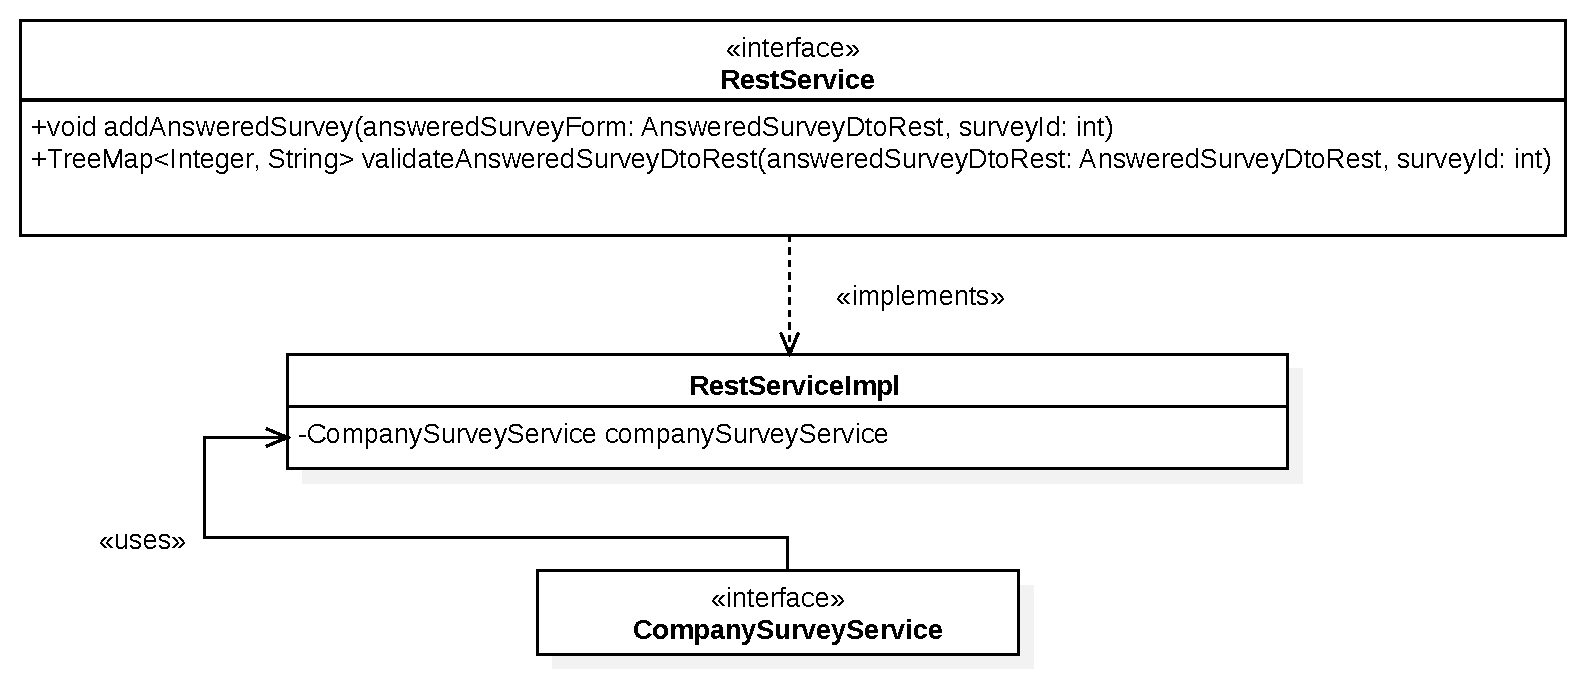
\includegraphics[scale=0.6]{rest_service.pdf}
  \caption{Diagram klas dla interfejsu serwisowego $RestService$}
\end{figure}
Powyższy diagram klas przedstawia diagram klas serwisowych obsługujących \textbf{REST Api}, które jest wykorzystywane przez aplikacje mobilna.
\begin{figure}[H]
  \centering
  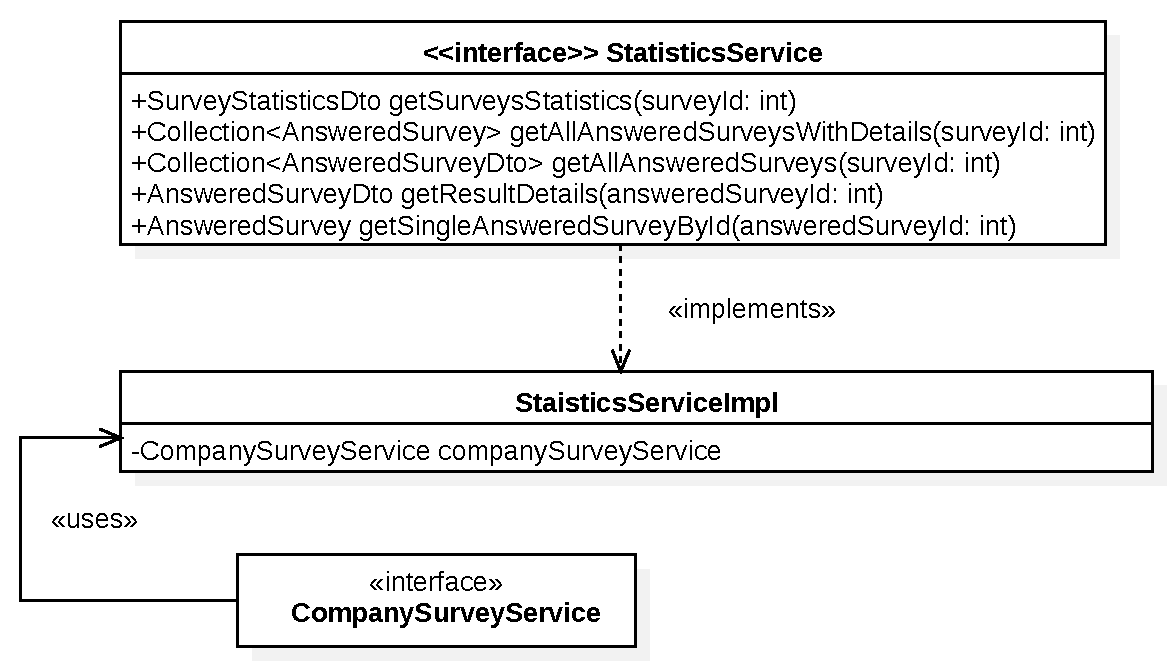
\includegraphics[scale=0.6]{statistics_service.pdf}
  \caption{Diagram klas dla interfejsu serwisowego $StatisticsService$}
\end{figure}
W powyżej przedstawionych klasach serwisowych obliczane są statystyki, które każdy użytkownik ze stworzonymi ankietami może przeglądać.
\begin{figure}[H]
  \centering
  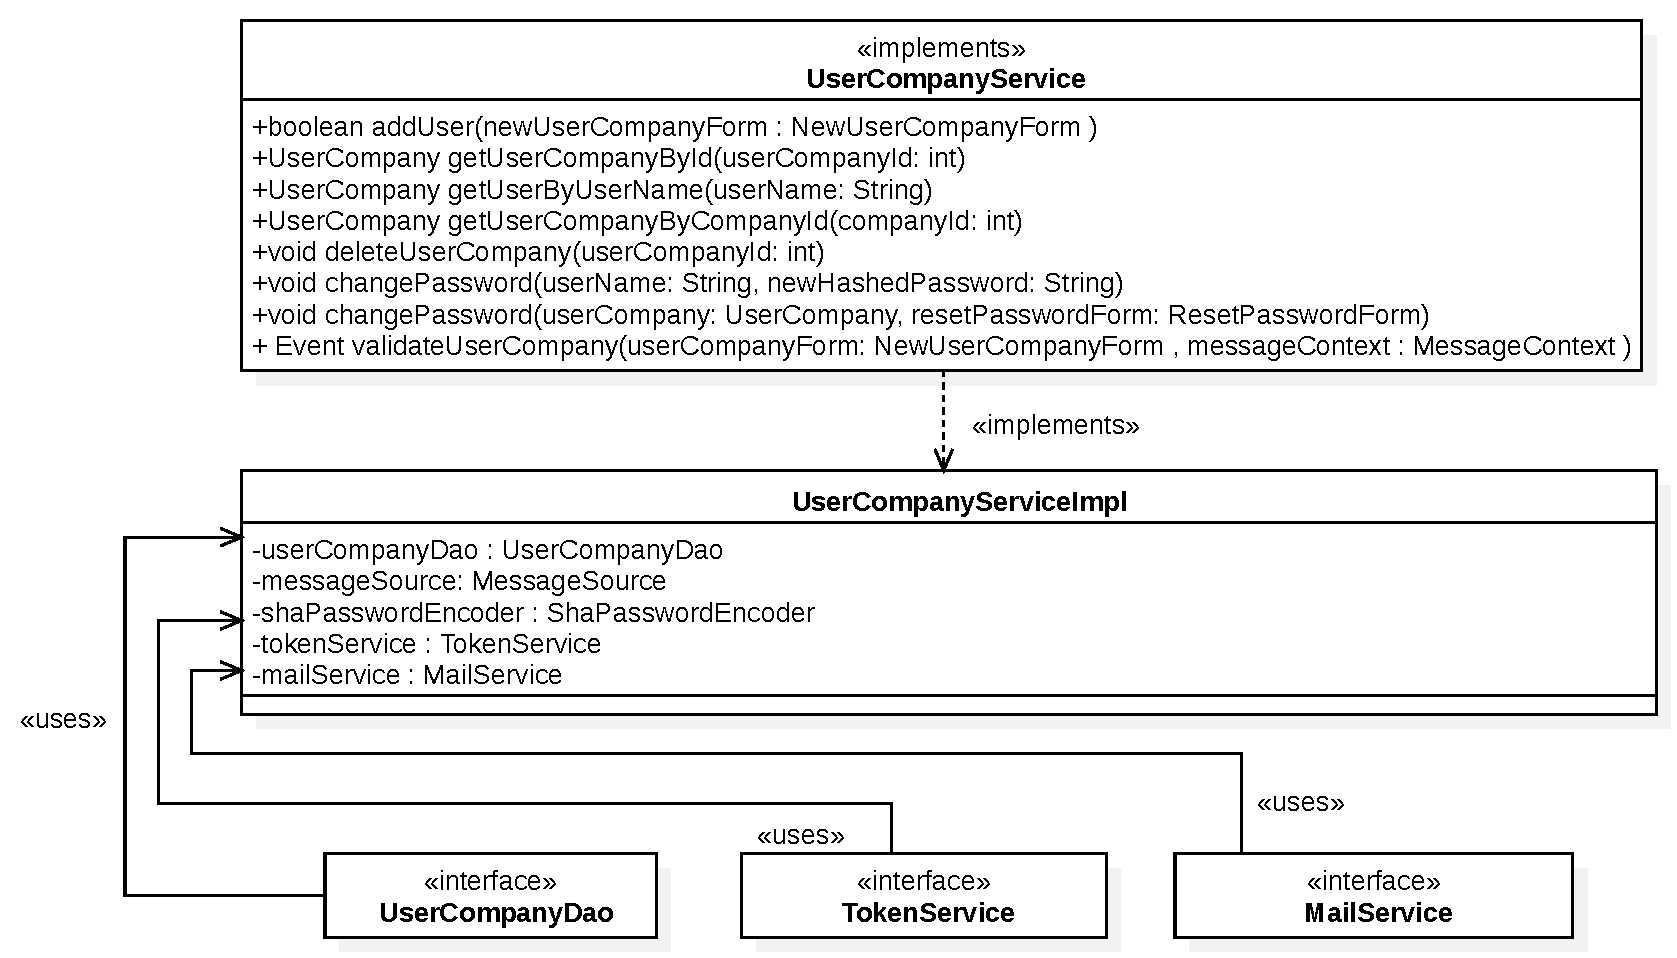
\includegraphics[width=12cm,height=17cm,keepaspectratio]{user_company_service.pdf}
  \caption{Diagram klas dla interfejsu serwisowego $UserCompanyService$.}
\end{figure}
Klasy serwisowe w diagramie powyżej odpowiadają za część funckjonalności związanej z kontem firmy, tj. edycja danych, rejestracja, logowanie, zmiana hasła itd.
\subsection{Diagramy aktywności}
\begin{figure}[htbp]
  \centering
  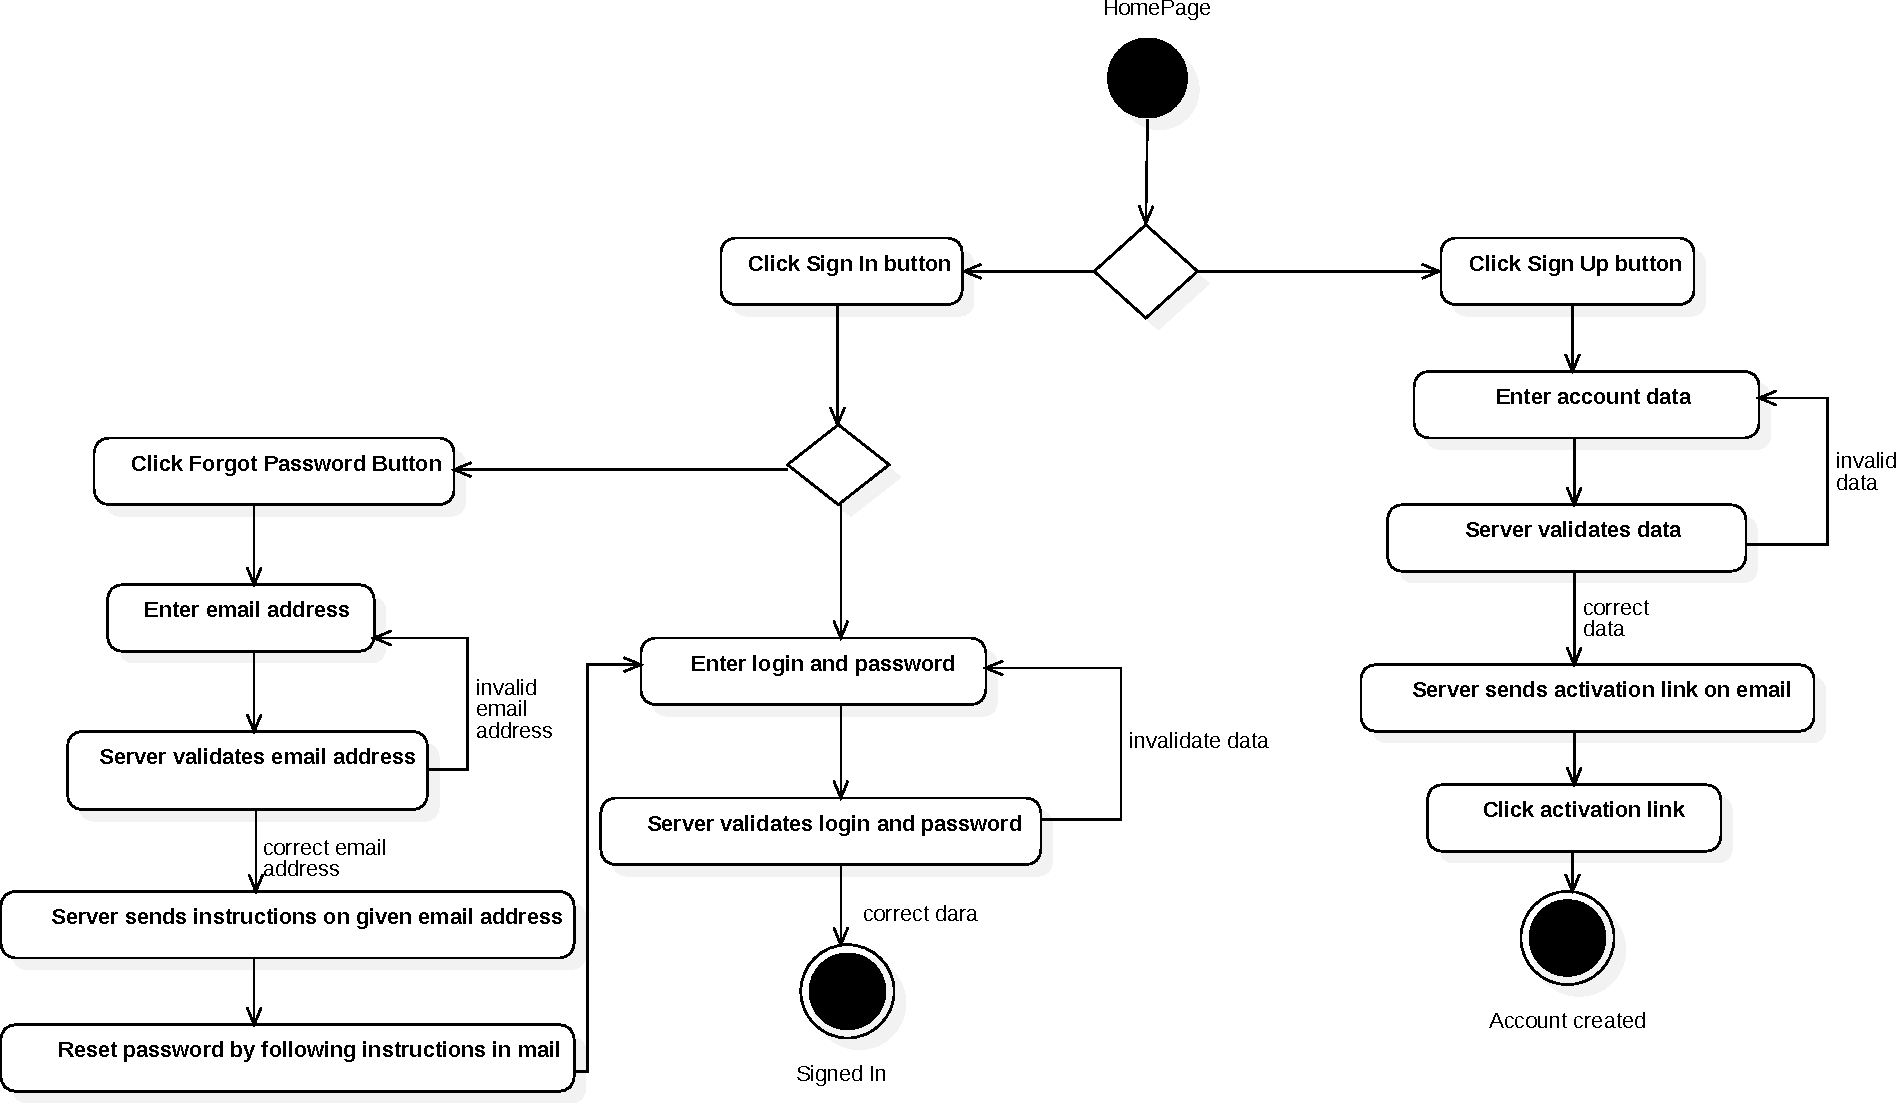
\includegraphics[scale=0.5]{activitySISU.pdf}
  \caption{Diagram aktywności dla logowania i rejestracji.}
\end{figure}

\paragraph{}
Powyższy diagram aktywności opisuje proces logowania i rejestracji w aplikacji webowej. Szczegółowy opis został przedstawiony w rodziale czwartym.

\begin{figure}[htbp]
  \centering
  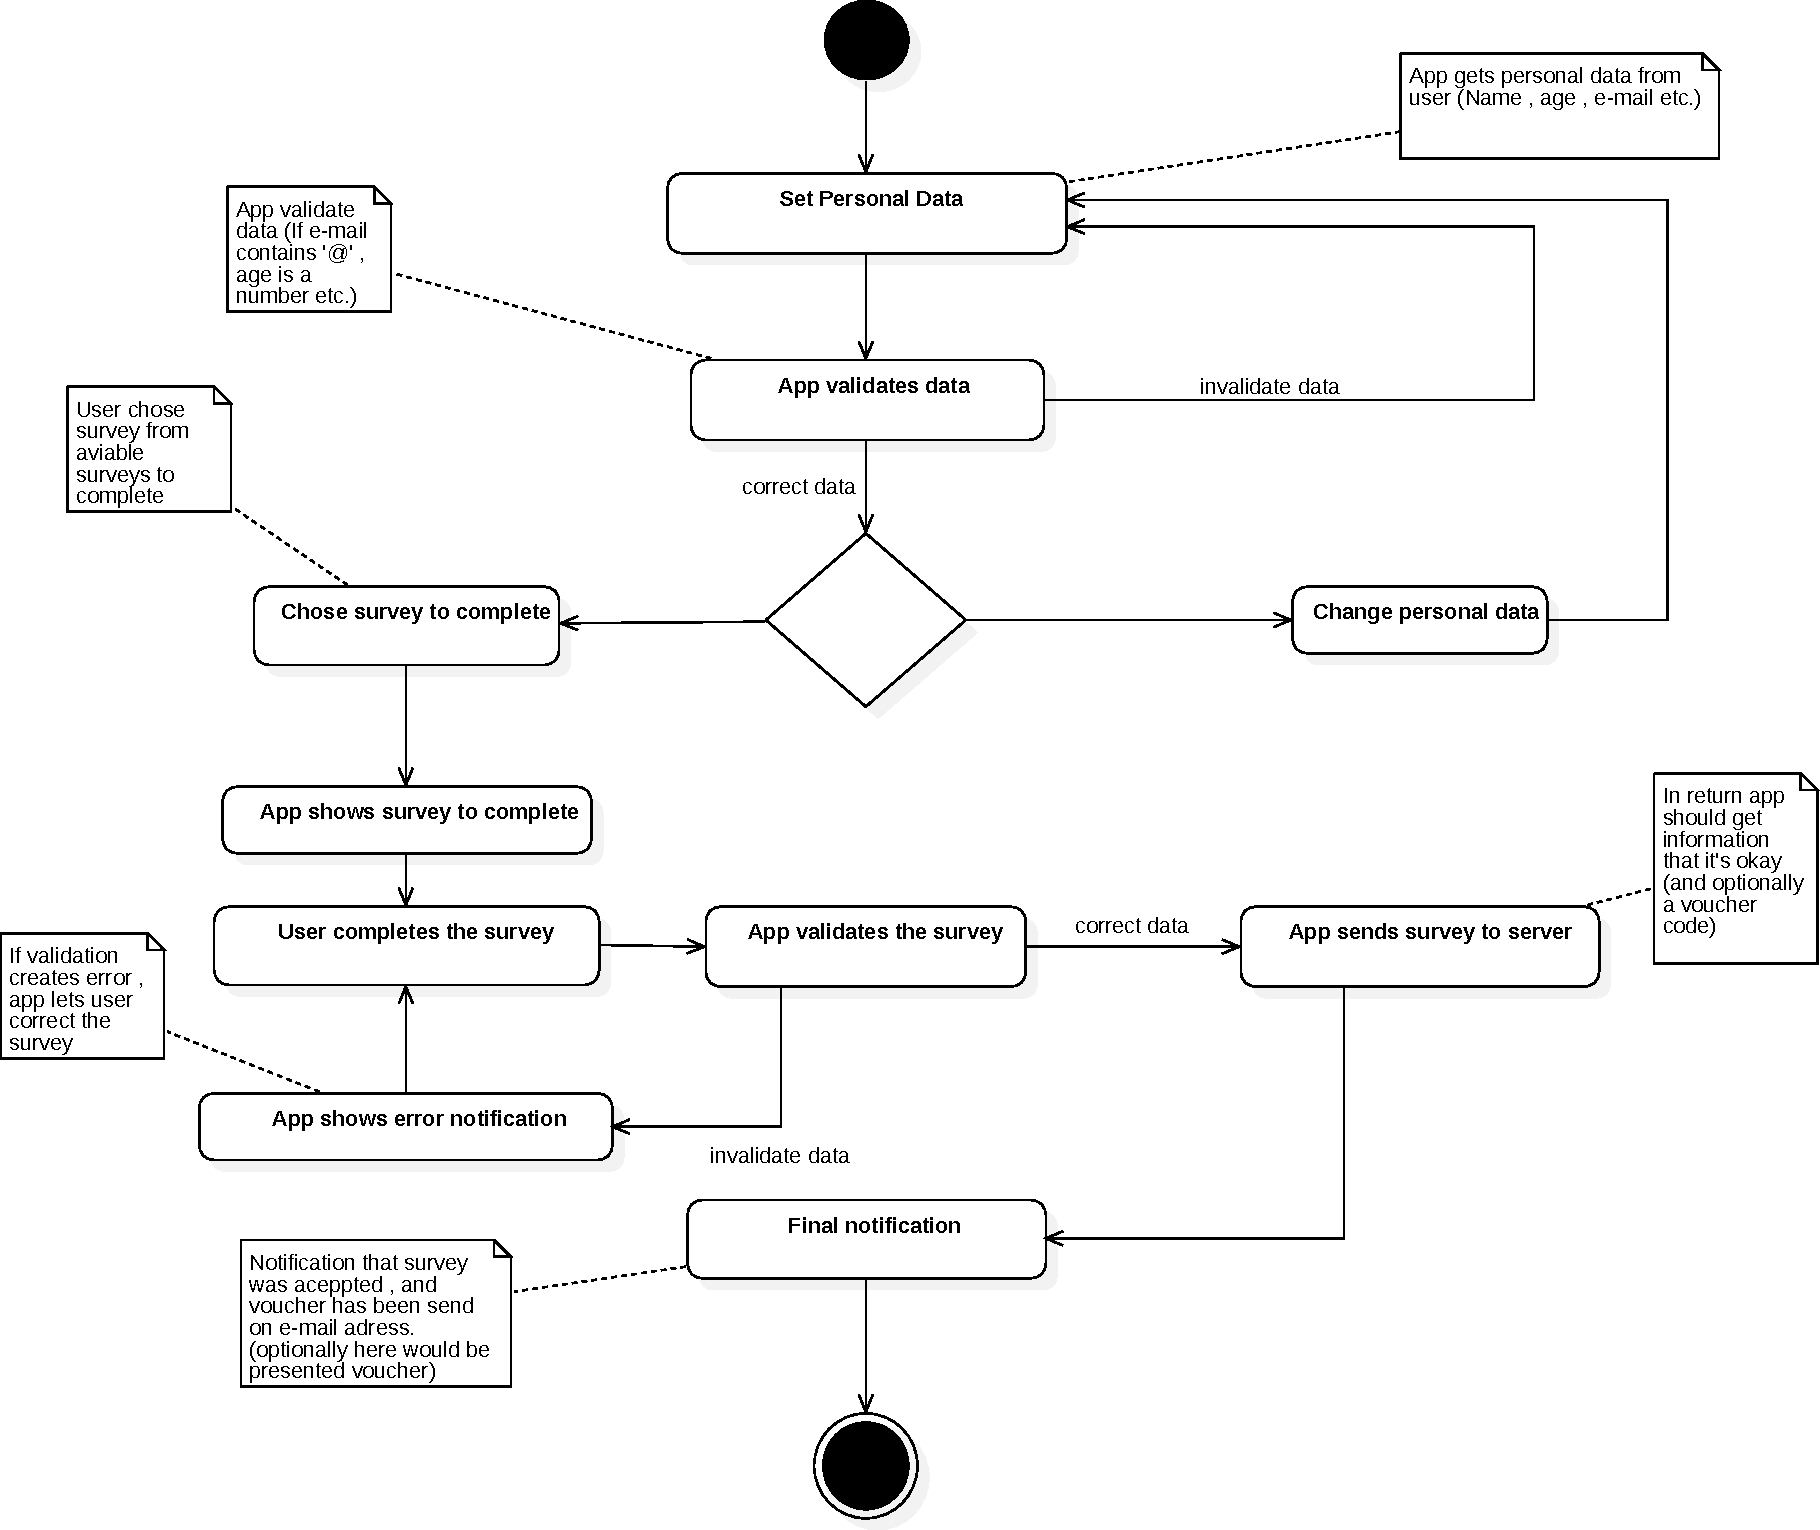
\includegraphics[scale=0.4]{MobileAppActivityDiagram.pdf}
  \caption{Diagram aktywności dla aplikacji mobilnej.}
\end{figure}

\paragraph{}
Głównym celem aplikacji mobilnej dla naszego serwisu, było umożliwienie użytkownikom w łatwy i prosty sposób uzupełnianie ankiet, oraz otrzymywanie kuponów w taki sposób, aby np. móc je okazać w sklepie na urządzeniu mobilnym. Przy pierwszym uruchomieniu aplikacji, użytkownik jest proszony o wprowadzenie danych dla celów statystyki. Jest to komfortowe rozwiązanie dla tych użytkowników, którzy planują korzystać z naszej aplikacji więcej niż raz. Aplikacja następnie wyświetla listę dostępnych firm oraz ankiet. Dzięki korzystaniu z aplikacji, użytkownik ma pod ręką możliwość wypełnienia dowolnej z możliwych ankiet w każdym momencie oraz dostęp do swoich wszystkich otrzymanych i niewykorzystanych kuponów.

\pagebreak
\subsection{Projekt bazy danych}
\begin{figure}[H]
  \centering
  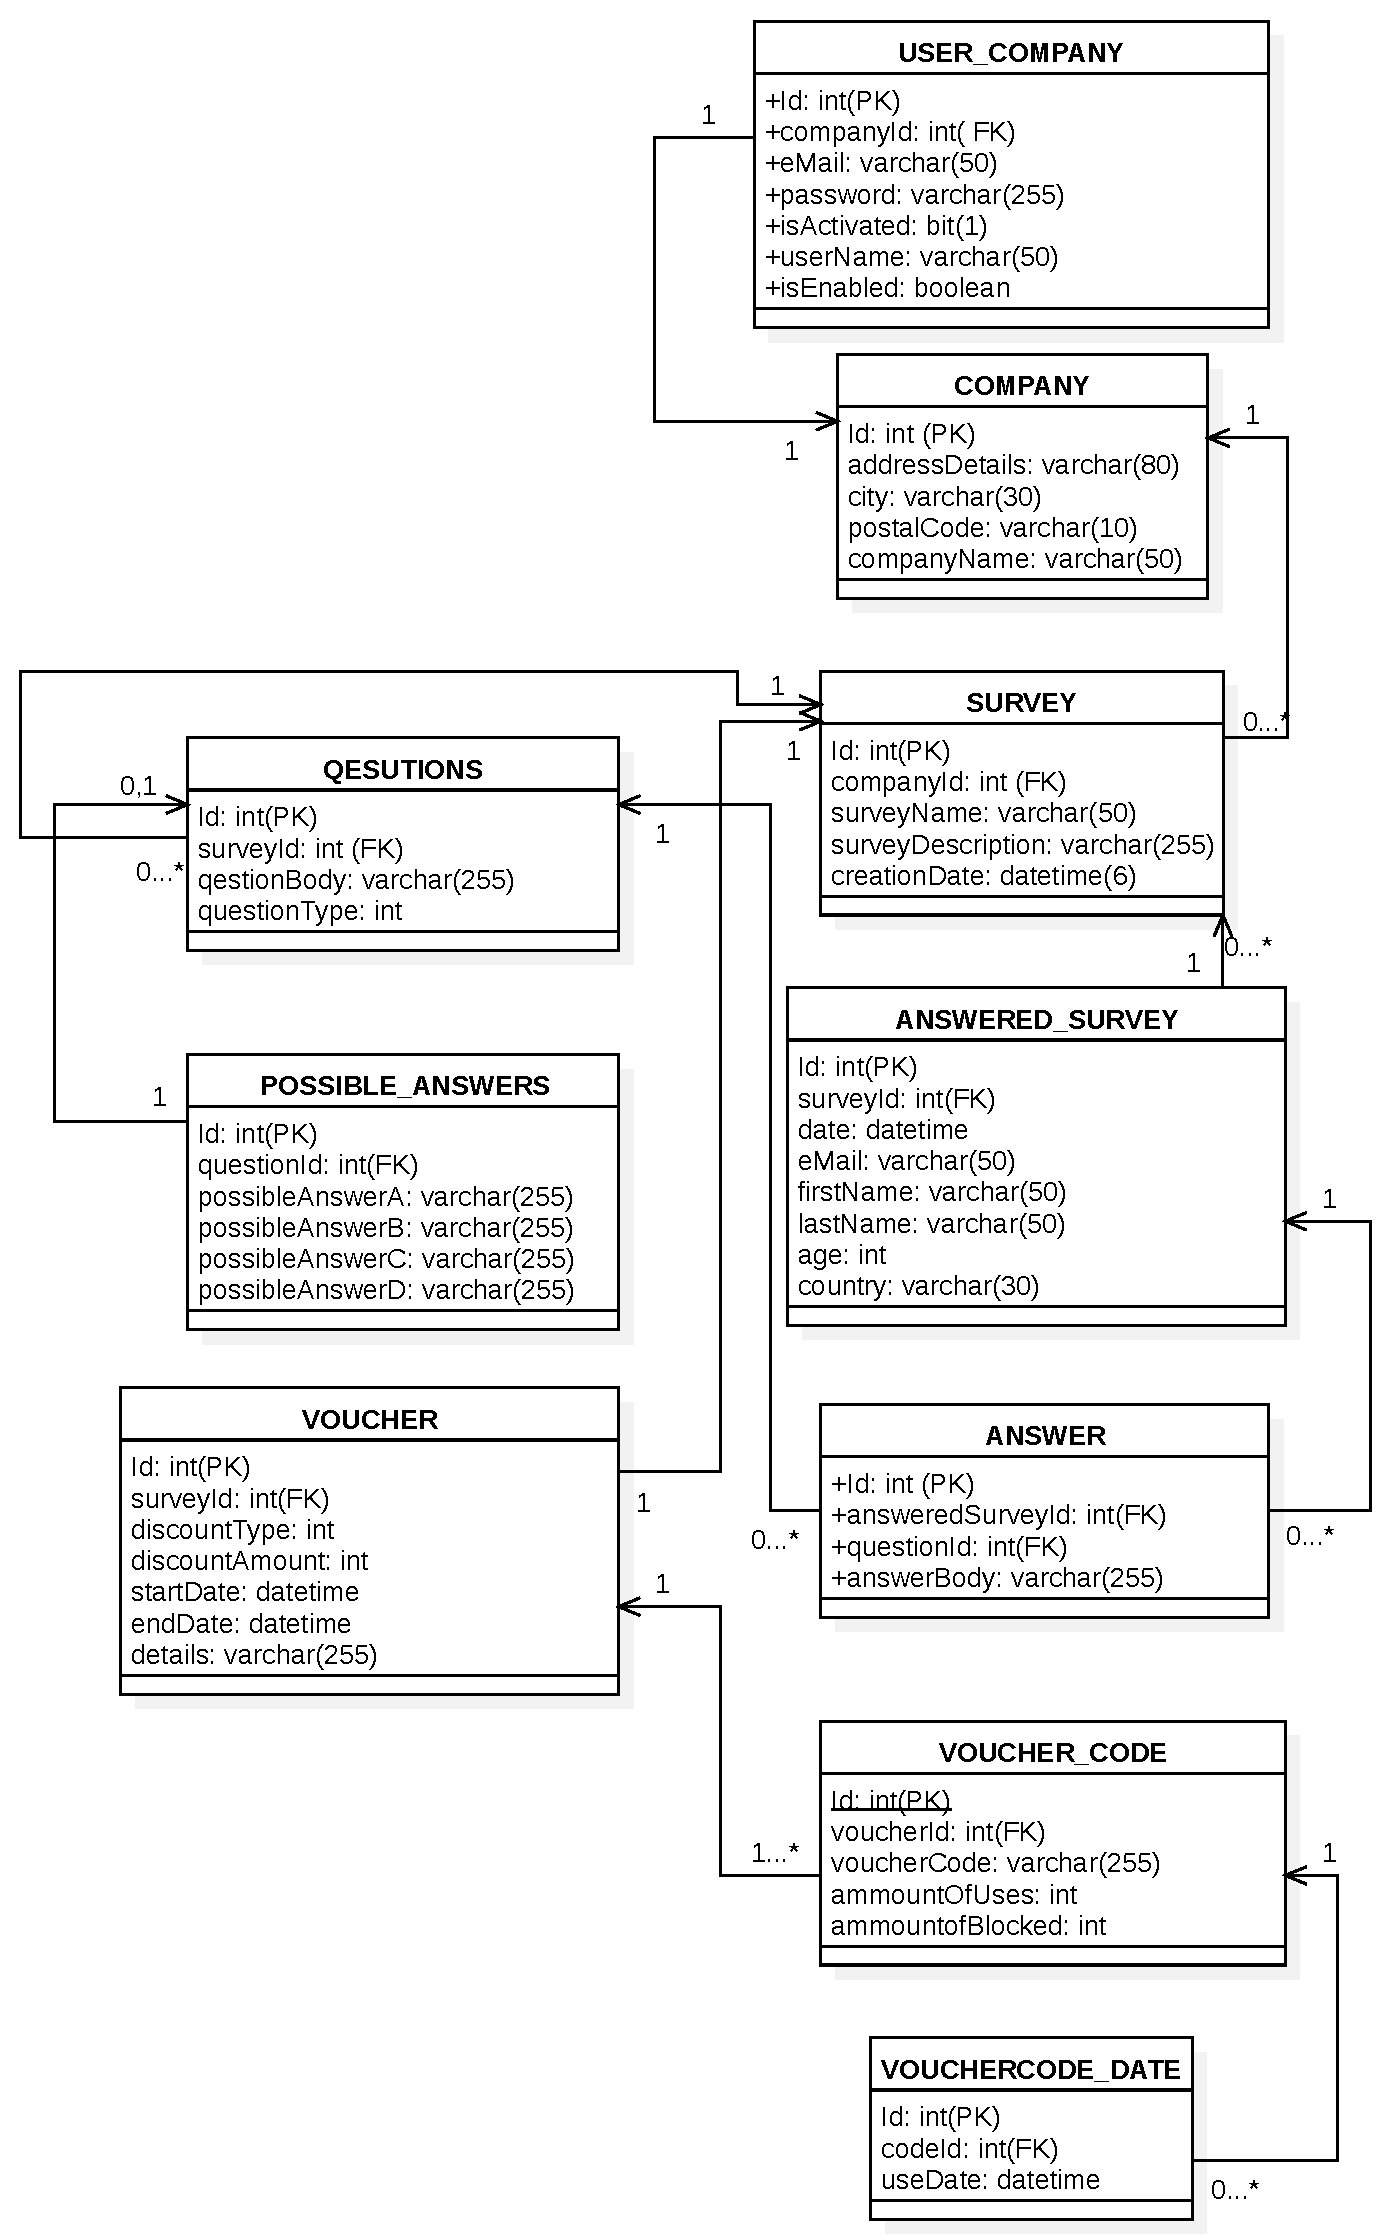
\includegraphics[scale=0.55]{db_diagram.pdf}
  \caption{Diagram klas przedstawiający baze danych systemu}
\end{figure}
W celu odpowiedniego zrozumienia struktury naszej aplikacji koniecznie jest zaznajomienie się kilkoma kluczowymi założeniami naszego systemu, którego miały bezpośredni wpływ na sposób w jaki zaprojektowaliśmy baze danych. Najważniejszym założeniem było przypisanie tylko i wyłącznie jednego typu kupony do jednej ankiety. Żadna ankieta może oferować tylko wyłacznie jeden typ kupony jako nagrodę za wypełnienie ankiety. Każdy voucher (który reprezentuje typ nagrody) może już miec przypisany więcej niż jeden kupon, każdy z nich może byc wielokrotnego użytku ( wtedy należy zaznaczyć jak wiele osób z niego może skorzystać) lub też jednorazowego użytku.

\paragraph{}
Równie ważnym założeniem było stworzenie tablicy \textbf{VoucherCode\_Date}, który odpowiada za ``blokowanie'' kupony na czas wypełnienia ankiet.
\subsection{Opis protokołów}
Ruch po naszej aplikacji ma miejsce przy użyciu protokołu \textbf{TLS}. Co ważne dostęp do każdej podusługi lub też podstrony naszego systemu wymaga połączenia zabezpieczonego, a użytkwonik chcący korzystać z naszej aplikacji przy użyciu protokołu \textbf{HTML} jest automatycznie przekierowywany na odpowiednią strone, która wykorzystuje już \textbf{TLS}. Podobno sytuacja ma miejsce z aplikacją mobilną, której połączenie z serwerem ma miejscu przy użyciu \textbf{TLS}.

\paragraph{}
Część aplikacji webowej dbająca o uwierzytelnianie	oraz autoryzacje (ang. authentication and authorization) przychodzących połączeń są filtry, które możemy uznać za protokół. Są one częścią \textbf{Servlet'ów}, która ma za zadanie jak sama nazwa wskazuje filtrować przychodzące zapytania, jak również w zależności od samego zapytania w odpowiedni sposób reagować. Informacje zawarte w zapytaniach oraz odpowiedziach serwera, które zostają dynamicznie przechowycone przez filtry są wykorzystywane między innymi do tego aby zidentyfikować autora zapytania (autoryzacja) i jeżeli będzie taka konieczność nadać mu odpowiednie uprawnienia (uwierzytelnienie). Jednym z zaimplementowanych przez nas zabezpieczeniem jest autoryzacja na poziomie metod serwisowych, jak również nadawanie ról użytkownikom w zależności od typu uprawnienień, które posiadają. Każdej osboie korzystającej z naszej aplikacji zostaje nadany unikatowy indetyfikator sesji, którym zostaje powiązany on i uprawnienia, które posiada. Właśnie te informacje wykorzystuje \textbf{The Security Filter Chain}, który jest częścią jednego z używanych przez nas narzędzi. Kiedy użytkownik legitymuje się swoim identyfikatorem sesji \textbf{The Security Filter Chain} (od tego momentu nazywany filtrem w celu zwiększenia czytelności tekstu) sprwadza w bazie danych czy istnieje już powiązane z tym identyfikatorem połączenie, w przypadku gdy zostanie to potwierdzone filter sprawdza jakie uprawnienia posiada to połączenie, skutkuje to powiązaniem uwierzytelnieniu zapytania przychodzącego do serwera, co następnie umożliwia wykorzystanie autoryzacji na poziomie metod, która sprawdza czy nasze uprawnienia są wystarczające.

\paragraph{}
Każdy użytkownik aplikacji webowej posiada odgórnie pewne uprawnienia, a w przypadku zalogowania się następuje dodatkowe uwierzytelnienie, gdzie jego identyfikator sesji wiązany z kontem do którego jest aktualnie zalogowany. To właśnie dzięki temu filter bezpieczeństwa potrafi jednoznacznie potwierdzić czy przychodzące zapytanie legitymujące się jedynie identyfikatorem sesji ma wystarczające uprawnienia do danej podusługi.

\paragraph{}
Ze względu na taki a nie inny sposób uwierzytelniania oraz autoryzacji konieczne również było użycie dodatkowego zabezpieczenia w postaci losowych tokenów chroniących przed atakami \textbf{CSRF} (ang. Cross-site request forgery), które w trakcie generowania zostają powiązane z identyfikatorem sesji, na którego życzenie zostały wygenerowane. Każdy użytkownik naszego serwisu podczas zapytań typu \textbf{POST} (sytuacja taka ma najczęściej miejsce podczas zatwierdzaniu różnego typu danych do serwera) musi ``wylegitymować się'' wygenerowanym wcześniej dla niego \textbf{CSRF tokenem} jak również identyfikatorem sesji, dopiero wtedy filter bezpieczeństwa zatwierdza takie zapytanie i przekazuje je do warstwy kontrolerów.

\paragraph{}
Częścią naszego systemu jest serwis mailowy, przez który jesteśmy w stanie komunikować się z klientami. Korzysta on z protkołu \textbf{STMP}.

\subsection{Możliwości rozwoju systemu}
\paragraph{Wdrożenie systemu}
Po zbudowaniu aplikacji i dodaniu artefaktu w \texttt{IDE} generujemy plik \texttt{JAR} lub \texttt{WAR}, który można wdrożyć w chmurze, np. \textit{Amazon Web Services}, które po skonfigurowaniu \texttt{Load Balancera} pozwoli na korzystanie z wersji \textit{live} aplikacji webowej.

Aby wdrożyć aplikację mobilną należy utworzyć konto deweloperskie w serwisie \textit{Google Play}, a następnie wygenerować klucze dla aplikacji mobilnej, powiązać je z aplikacją mobilną i przesłać pliki aplikacji do serwisu \textit{Google'a}.

\paragraph{}
System gwarantuje całkowite pokrycie wszystkich założeń funkcjonalnych i niefunkcjonalnych. Możliwe jest jednak rozwój systemu o kolejne funkcjonalności. Bezpośrednimi funkcjonalnościami, które w łatwy sposób mogą zostać zbudowane na bazie istiejących rozwiązań są między innymi powiązanie kodów promocyjnych kuponu z kodami QR. Aby wprowadzić taką funkcjonalność będzie należało dodać kolejne pole w klasie odpowiadającej w modelu za kupon, które będzie przechowywać kod QR. Kod ten może być w łatwy sposób zwracany do użytkownika i wyświetlany na ekranie wraz z pozostałymi szczegółami kuponu. Kolejną funkcjonalnością, o którą może zostać rozbudowany system jest wprowadzenie algorytmu decydującego o zdobywaniu kuponu. Kupony mogą być wydawane co piąte wypełnienie ankiety, z dowolnym prawdopodobieństwem lub w ogóle. System jest napisany w sposób, który umożliwia modyfikacje serwisu bez konieczności przeprojektowania pozostałej logiki. System charakteryzuje się wysoką spójnością i niskim sprzężęniem.